The aim of the proposed system is to investigate the implementation of \gls{coap} 
on a \gls{rpi} and how \gls{coap} can be 
used to transmit data to the cloud. 

To achieve this a \gls{coap} endpoint will need to be created on the \gls{rpi}. 
The \gls{rpi} will collect sensor data at intervals and store them 
locally on the device. The \gls{rpi} will act as a \gls{coap} server that will 
respond to \gls{rest} GET requests with the sensor data and the time
the reading was taken in a \gls{json} format.

The clouds responsibility will be to send the GET requests to the \gls{coap} 
endpoint hosted on the \gls{rpi} and to receive and store the data
returned. The cloud should send a confirmable request to the \gls{coap} endpoint. 
The \gls{coap} endpoint should then respond with an acknowledgement. 
If the data is available, the data should be ``piggybacked'' to this response, as 
shown in Figure \figref{fig:coap_get_piggy}, if not the data should be 
returned in a confirmable message containing the data.
 In this case the cloud client will then send it's own acknowledgement message to 
 the \gls{coap} endpoint. This is shown in  \figref{fig:coap_get_delayed}.

\begin{figure}[H]
    \centering
    \makebox[1\textwidth]{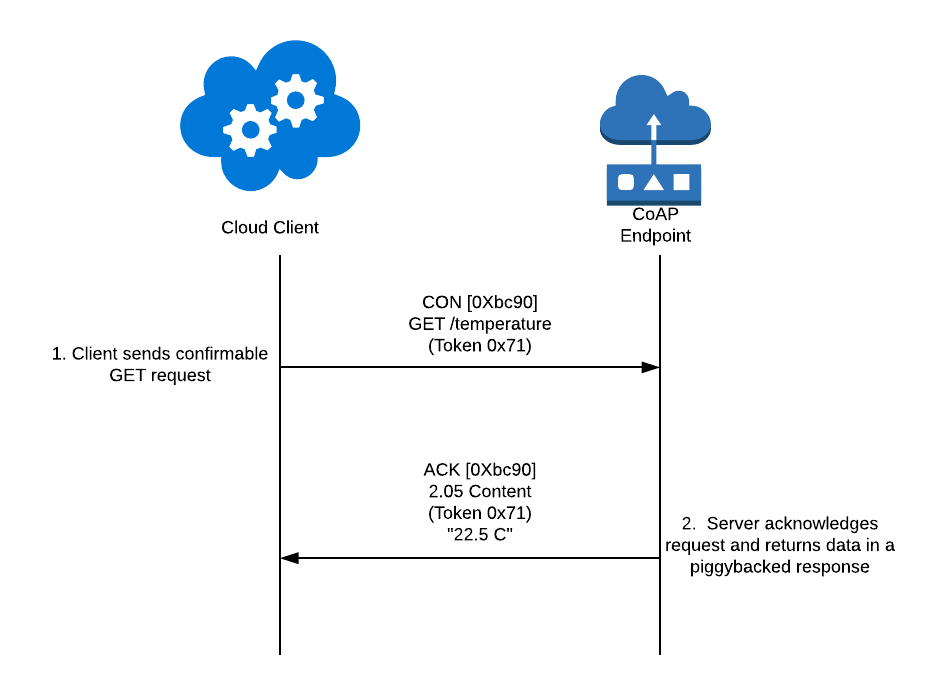
\includegraphics[width=1\textwidth]{assets/coap_get_request.png}}
    \caption{\label{fig:coap_get_piggy} Example \gls{coap} GET request with piggybacked response. \citep{shelby_constrained_2014}}
\end{figure}

With \gls{coap} endpoints acting as both a client, that sends requests, and a 
server implementation of \gls{coap} will be needed 
in each the \gls{rpi} and the cloud platform. The \gls{rpi} will then regularly 
retrieve readings from the sensor and send a POST request 
at intervals to the cloud \gls{coap} endpoint. This approach will be contrasted 
with the cloud server observing the \gls{rest} endpoint on the \gls{rpi}.
The results of both approaches will be evaluated.

\begin{figure}[H]
    \centering
    \makebox[1\textwidth]{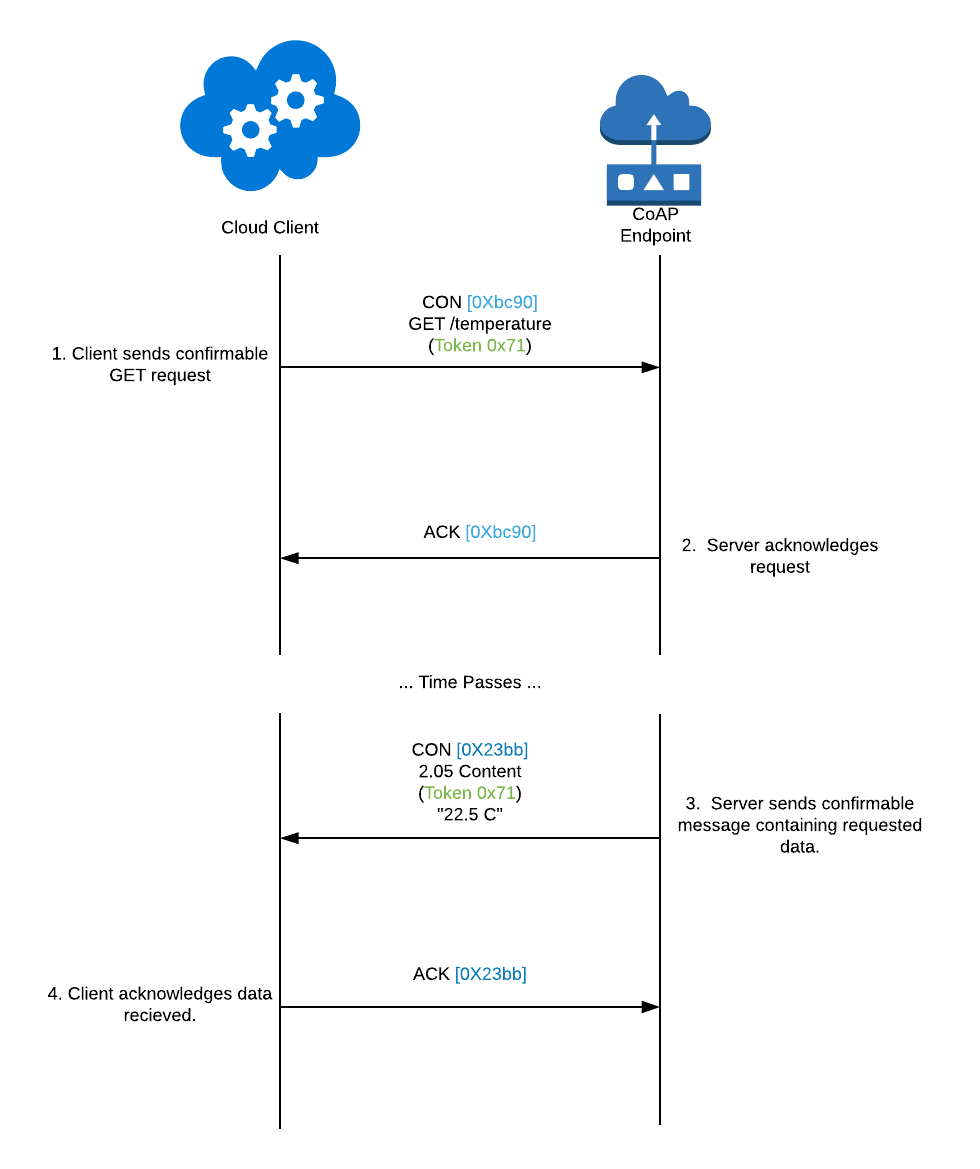
\includegraphics[width=1\textwidth]{assets/coap_get_delayed.png}}
    \caption{\label{fig:coap_get_delayed} Example \gls{coap} GET request without 
    piggybacked response. \citep{shelby_constrained_2014}}
\end{figure}
